\subsection{Utilização no LIMS Flux}

O LIMS Flux foi utilizado para implementação dos recursos de workflows dinâmicos e da agregação de múltiplos BPMs para troca de informações entre eles. Sua utilização foi feita pela facilidade na criação de workflows dentro do próprio software e a alta personalização disponibilizada.

Como estes recursos alteram como a visualização de um BPM ocorre, foram necessário ajustes para que a implementação de tais recursos fosse feita de maneira correta e consistente, sem que a alteração na visualização deixasse o LIMS com vulnerabilidades de segurança e que as informações estivessem sempre disponíveis quando necessário.

\subsection{Alterações feitas para workflow dinâmicos}

Para que o Flux pudesse focar em uma atividade dentro do workflow, alteramos a definição de instância do programa. Anteriormente, instâncias eram definidas como o inicio do fluxo de trabalho do usuário para execução do BPM.

Com a implementação de workflows dinâmicos, foi necessário a utilização de instâncias como o ponto de partida de execução do usuário naquele momento, e não necessariamente o inicio do fluxo de trabalho. As instâncias agora demonstram, como ponto inicial, a atividade focada pelo usuário.

No software, instâncias ainda são criadas apenas para a atividade original, mantendo a ordenação do BPM, mas a disponibilização de informações é feita de maneira dinâmica, criando uma instância temporária onde a atividade inicial é a atividade selecionada pelo usuário, disponibilizando esta atividade centralizada como ponto de partida para sua execução.

Para selecionar qual atividade inicial será utilizada na visualização atual, foi alterada a interface para adicionar um seletor de atividades, disponibilizando todas as atividades que o usuário tem permissão de acessar em uma lista ordenada pelo nome da mesma. Nele, temos o nome de todas as atividades do workflow selecionado que o usuário tem a permissão de visualizar.

Caso o usuário não selecione nenhuma atividade, a atividade inicial utilizada será a padrão, deixando o workflow na visualização padrão. Exemplos para esta funcionalidade são mostrados na seção~\ref{sec:dinamic_workflows_examples}.

A árvore de atividades também teve de ser alterada, com a criação de novos tipos de atividades: Atividades pai, ou atividades anteriores. Neste tipo de atividade (Identificados pela cor azul na figura~\ref{fig:centrare_tree_normal_altered}), não é possível executar novas atividades, sendo existentes apenas por motivos de disponibilização de informações pertinentes à execução atual.

Foi necessário a criação deste novo tipo de atividade para disponibilizar informações de atividades anteriores para o usuário, já que as informações podem ser pertinentes para o usuário.

Na mesma figura~\ref{fig:centrare_tree_normal_altered} temos as informações do paciente como primeira atividade da visualização original, podendo ser necessária para preenchimento de próximas atividades da atividade selecionada ``Cirurgia de Nariz''.

\begin{figure}
    \centering
    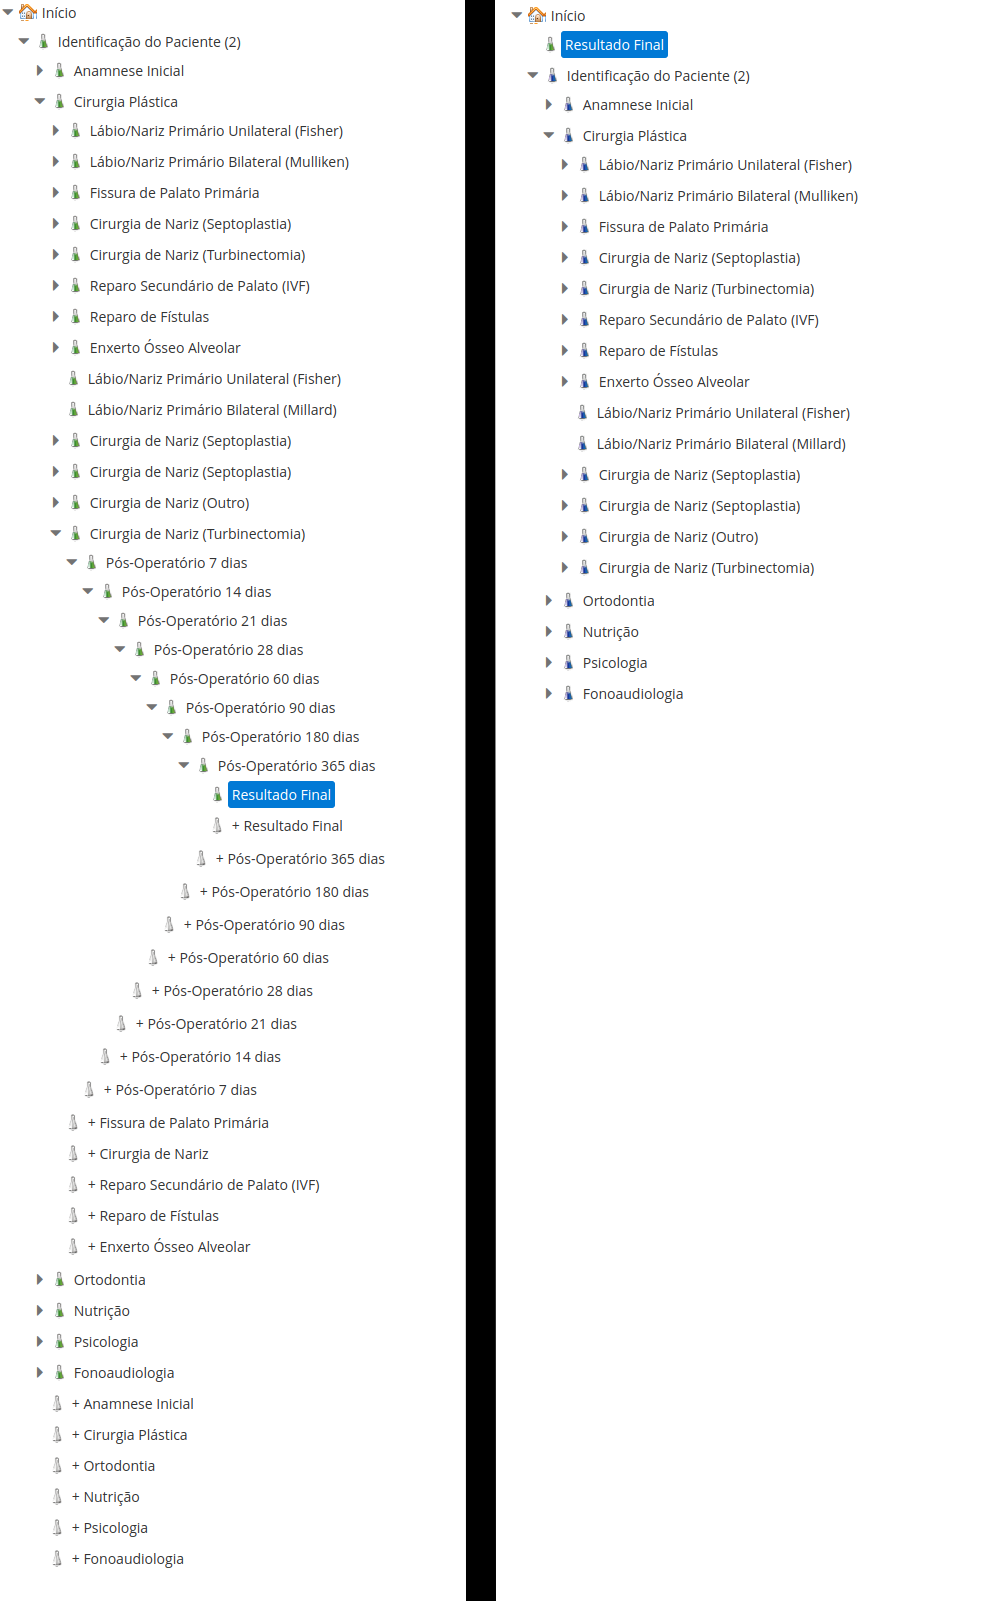
\includegraphics[height=1\textwidth]{imgs/CENTRARE/arvoreNormalEAlterada.png}
    \caption{Imagem demonstrando a árvore de atividades no software original (Esquerda) e a árvore de atividades alterada (Direita). Como podemos ver, a atividade selecionada na esquerda que está no meio do workflow é a mesma atividade selecionada na direita, que agora virou a atividade focada por seleção do usuário. Atividades pai são demonstradas em azul, disponibilizando todas as informações existentes mesmo com a alteração do foco do workflow.}
    \label{fig:centrare_tree_normal_altered}
\end{figure}

\subsubsection{Como funciona}

Quando o usuário seleciona a atividade desejada para ser a atividade inicial, a árvore de atividades é reajustada para que a atividade selecionada seja o foco principal da instância.

Para que isso ocorra, é necessário que a atividade selecionada se torne a atividade inicial, continuando com suas atividades filhas originais mas ganhando uma nova atividade filha: Sua atividade pai. As atividades que eram pais da atividade selecionada se tornam filhas da mesma para que essas informações estejam disponíveis para acesso e para manter a conformidade com a modelagem do BPM já existente.

Para isso, pode-se dizer que ocorre um ``giro'' na árvore de atividades para a direita, tendo todas as atividades anteriores como atividades filhas da selecionada, mantendo a sub árvore de atividades originais intacta. Podemos ver esta característica na figura~\ref{fig:primeira_implementacao}.

No Flux, esta funcionalidade faz com que atividades pai tenham uma cor diferente na interface do usuário (em azul na figura~\ref{fig:centrare_tree_normal_altered}) para que seja claro que as atividades vistas pelo usuário são atividades pai da atividade selecionada. Também é desabilitado a execução de novas atividades a partir das atividades pai.

\subsubsection{Exemplos} \label{sec:dinamic_workflows_examples}

Como exemplo, utilizaremos o workflow modelado para o CENTRARE, que é um fluxo de trabalho para o Centro de Tratamento e Reabilitação de Fissura Labiopalatal e Deformidade Craniofacial do hospital da baleia, em Belo Horizonte.

Nele, é feito o acompanhamento de pacientes desde o nascimento até a adolescência por múltiplos médicos de diferentes áreas da saúde como odontologia, cirurgia plástica e psicologia. Este fluxo de trabalho é utilizado para o tratamento de lábios leporinos em crianças recém nascidas, com acompanhamento completo pós cirúrgico, familiar e nutricional.

Como este workflow é muito profundo e tem informações de anos acumuladas em um mesmo sistema, ele foi selecionado para a aplicação desta implementação para verificar que as informações ficam mais facilmente disponíveis para os usuários que o utilizam.

Podemos ver a diferença da figura de visualização padrão do fluxo de trabalho (\ref{fig:normalInstance}) e visualização alterada (\ref{fig:changedInstance}). Na primeira imagem, temos uma tabela para seleção de instâncias sem alteração da visualização do workflow. Nela, cada linha na tabela disponibiliza um paciente diferente para seleção.

Na segunda imagem, foi selecionado a atividade ``Cirurgia de Nariz'', disponibilizando todas as cirurgias de Nariz realizadas em todos os pacientes. Em cada linha é disponibilizado certos atributos para visualização para identificar a atividade desejada para obtenção de informações (como visto na figura~\ref{fig:cttx_eqp_calibracao_focada}, cada linha disponibilizando a data de execução da atividade, data de calibração, nome do equipamento e POP).

\begin{figure}
    \centering
    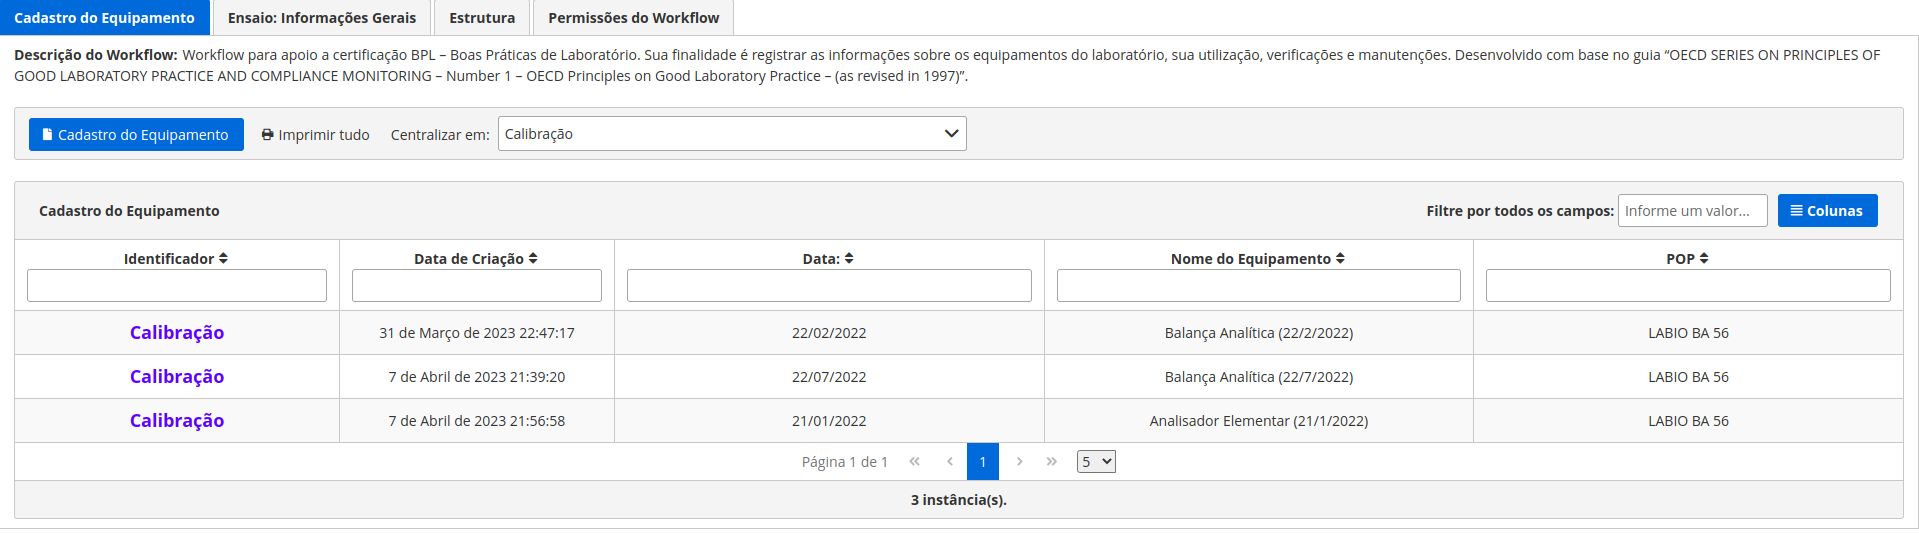
\includegraphics[width=1\textwidth]{imgs/CTTX-EQP/cttx_eqp_calibracao_focada.png}
    \caption{O workflow CTTX-EQP com a atividade compartilhada ``Calibração'' focada.}
    \label{fig:cttx_eqp_calibracao_focada}
\end{figure}

Existem mais atividades do tipo ``Cirurgia de Nariz'' porque, seguindo a modelagem do workflow CENTRARE, existe o cadastro de um paciente que, por sua vez, pode ter feito uma ou mais cirurgias de nariz. Para identificar qual atividade pertence a qual paciente, pode ser adicionado um atributo na atividade que recebe como valor o nome do paciente (ou um identificador único), deixando mais rápido para o usuário identificar a qual instância do workflow original aquela atividade pertence. Esse tipo de identificação foi utilizado no workflow CTTX - EQP que será explicado nas próximas seções.

\begin{figure}
    \centering
    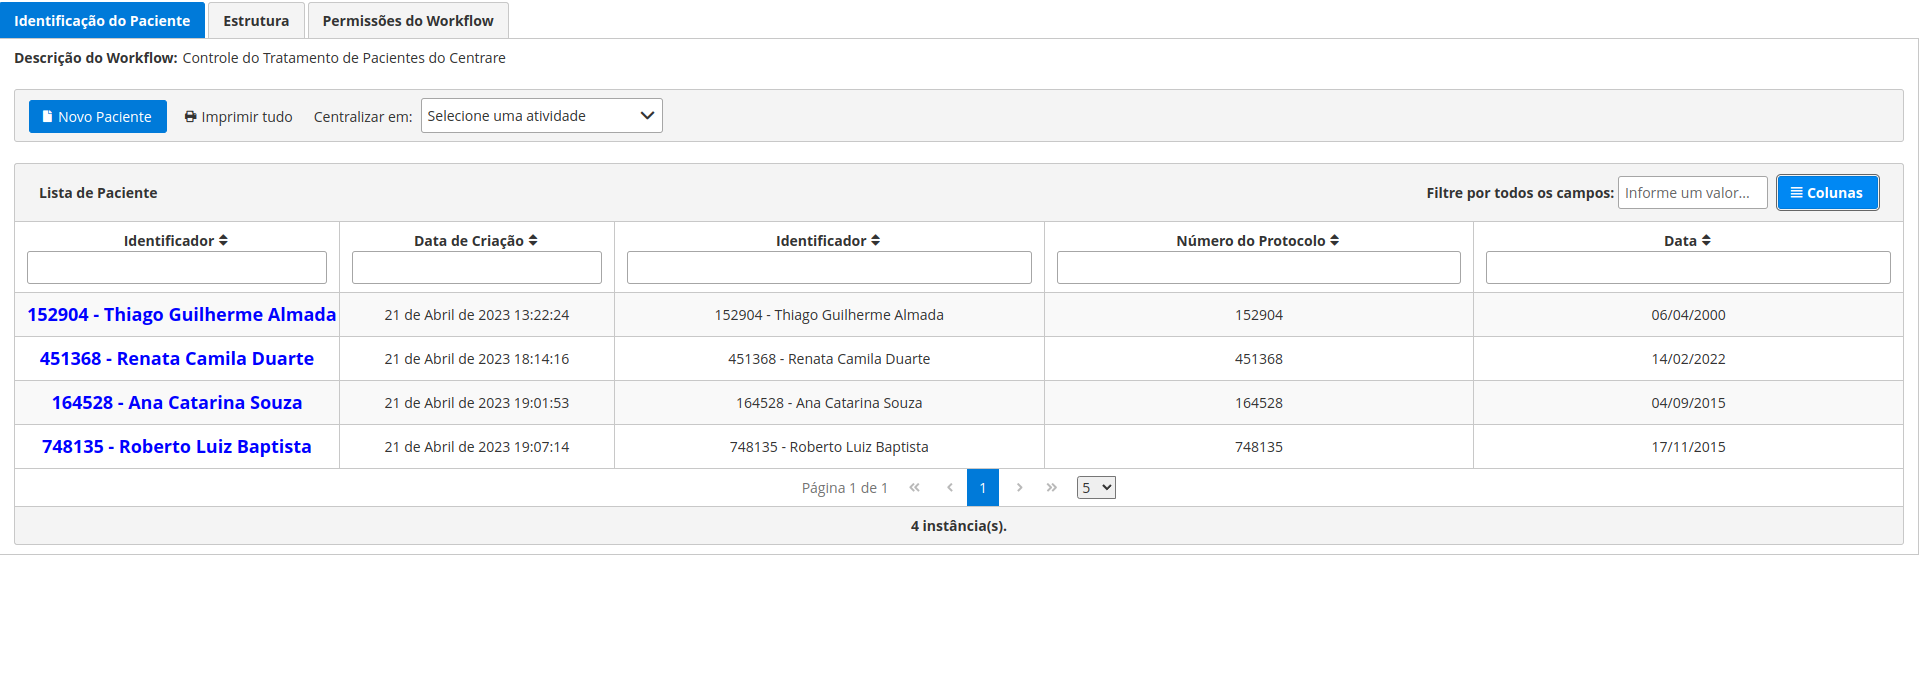
\includegraphics[width=1\textwidth]{imgs/CENTRARE/instanciaNormal.png}
    \caption{Workflow padrão do CENTRARE, sendo sua centralização feita na atividade inicial de ``Identificação do Paciente''}
    \label{fig:normalInstance}
\end{figure}

\begin{figure}
    \centering
    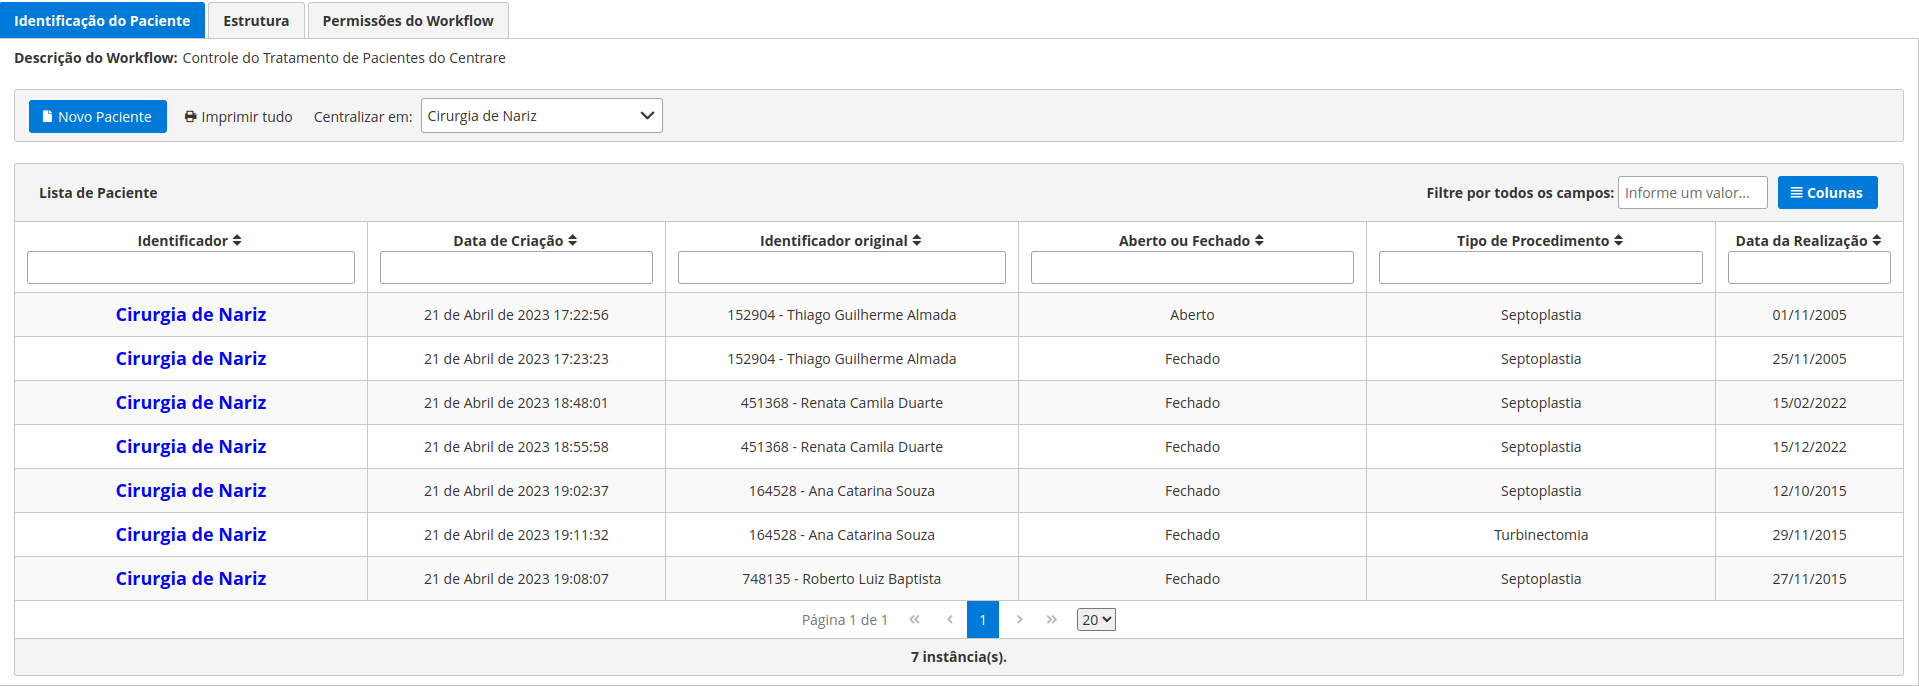
\includegraphics[width=1\textwidth]{imgs/CENTRARE/instanciaAlterada.png}
    \caption{Workflow com visualização centralizada na atividade ``Cirurgia de Nariz, disponibilizando informações da atividade como ``Cirurgião'', ``Aberto ou Fechado'' e ``Topo de Procedimento''}
    \label{fig:changedInstance}
\end{figure}

Ao acessar o workflow, podemos ver pela figura~\ref{fig:centrare_tree_normal_altered} a alteração da árvore do workflow, disponibilizando as atividades anteriores (em azul) para acesso do usuário, disponibilizando informações de outras atividades caso necessário (como a identificação do paciente) e disponibilizando o acesso mais efetivo de atividades filhas dessa atividade.

Esta funcionalidade acelera o acesso à atividades profundas (como a ``Cirurgia de Nariz'' citada) já que a atividade e seus atributos ficam disponíveis na tabela de seleção de instâncias para que possam ser visualizadas, facilitando a seleção pelo usuário.

No caso de um gerente que quer saber quantas cirurgias foram feitas, selecionar a atividade disponibiliza todas as executadas para o usuário, acelerando a coleta de informações. Além disso, caso ele queira selecionar apenas cirurgias de um certo tipo, pode apenas filtrar pelo atributo de Tipo de cirurgia disponível na tabela de seleção de instâncias, facilitando a seleção da atividade buscada.

\subsection{Alterações feitas para múltiplas atividades iniciais}

Enquanto a BPMN permite múltiplas maneiras de iniciar um processo, ela permite apenas uma atividade inicial em um diagrama de processo, representado por um único evento de início.

Como uma organização pode ter múltiplas equipes trabalhando em focos diferentes, é necessário a divisão em diversos workflows para que todos os processos estejam modelados para que fluxos de trabalho possam ser diagramados e executados.

Como um mesmo workflow pode ter troca de informações com alguma parte de outros workflows, foi idealizado uma nova funcionalidade para um workflow no Flux: Múltiplas atividades iniciais que compartilham atividades entre instâncias no meio de sua execução.

Cada possível atividade inicial do workflow pode ser utilizada para criar uma instância diferente do workflow, já que cada uma dessas atividades representa um tipo de execução diferente do workflow (na figura~\ref{fig:segunda_implementacao}, uma atividade inicial é para cadastro de pacientes e a outra para cadastro de técnicos de laboratório).

Com um workflow com múltiplas atividades iniciais, é possível ter atividades que, ao serem executadas, serão disponibilizadas para outros usuários que utilizam este workflow, independente da instância que estiverem executando. Assim, usuários que estão executando atividades em uma parte do workflow (partindo de uma atividade inicial) compartilham informações com outros usuários (partindo de outra atividade inicial).

Com a execução de dois workflows agregados, cada execução iniciando de uma atividade inicial diferente, é possível o compartilhamento das atividades que contém um processo idêntico entre os dois workflows agregados, disponibilizando as informações para as instâncias selecionadas.

Desta forma, aumenta-se a integração do sistema por haver a troca de informações entre processos de trabalho diferentes dentro de uma mesma organização, disponibilizando a cooperação entre usuários do mesmo sistema.

\subsubsection{Como funciona}

Para compartilhar atividades entre múltiplos workflows, é necessário que estes workflows estejam juntos em uma mesma modelagem com múltiplas atividades iniciais.

Para isso, foi alterado o editor de workflows já existente no Flux para que fosse possível criar múltiplas atividades iniciais, uma atividade inicial para cada workflow agregado.
Os workflows não precisam ter atividades compartilhadas para estarem juntos, eles funcionarão como workflows normais, com criação de instâncias e atividades da mesma maneira, apenas estando sob o mesmo nome de workflow e dentro da mesma interface que disponibiliza as informações de um workflow, disponibilizando recursos como busca de informações e geração de relatório dentro do mesmo workflow.

Quando uma atividade deve ser compartilhada entre workflows, é necessário cria-la como filha de uma das atividades que a utilizarão. Logo após a criação da atividade, é necessário criar transições entre todas as atividades pai para que tenham a atividade compartilhada disponível para execução (figura~\ref{fig:transition_ref}).

Existem dois tipos de compartilhamento: Um compartilhamento geral, onde a atividade será compartilhada entre todas as instâncias existentes assim que ela for criada e um compartilhamento seletivo, onde o usuário escolhe qual instância receberá as informações da atividade executada.

No caso do compartilhamento geral, ele é necessário pois atividades podem ser executadas antes de uma instância existir, como por exemplo no workflow de Citotoxicidade (CTTX): Um equipamento pode existir antes de um ensaio de citotoxicidade ser executado.

Para o compartilhamento seletivo, ele é necessário porque em um pedido de exame, o envio do exame deve ser feito para um laboratório específico e não pode aparecer para outros laboratórios, sendo necessário a seleção de qual laboratório receberá o compartilhamento da atividade.

Nos dois casos, o compartilhamento de atividades tem uma ligação forte com o sistema de permissões. A disponibilização de atividades filhas da atividade compartilhada deve ser controlado pelos administradores do workflow, alterando as permissões de visualização das atividades. Caso contrário, todas as atividades e as informações contidas nelas serão compartilhadas.

Com isso, é possível montar o workflow de forma a disponibilizar a requisição de dados entre usuários. Cada usuário fica responsável pela execução de uma atividade específica do workflow, executando atividades que estes usuários tenham permissão para executar. Quando um usuário não tem permissão para executar uma atividade e outro usuário tem, atividades filhas só ficam disponíveis após o usuário com permissão executar a atividade, permitindo a troca de informações entre os usuários. A colaboração é essencial para a execução do workflow.

\subsubsection{Exemplo de pedido de exame}

Vamos utilizar o exemplo de um pedido de exame em um workflow médico e o recebimento deste pedido de exame e execução do mesmo.
Um médico cria uma instância de paciente, cadastrando-o e seguindo o fluxo de trabalho comum de atendimento.
O laboratórios do hospital também tem seu próprio workflow, onde são cadastrados equipamentos para análise de amostras.
Antes, os workflows ficariam separados, sem comunicação entre eles.

Com o novo recurso implementado, os workflows podem compartilhar atividades como o pedido de exame: O médico tem a permissão de executar o pedido de exame, mas ele não aprova a atividade. Quem irá aprovar a atividade é o técnico de laboratório.

O técnico de laboratório recebe uma notificação que a atividade foi executada e pode aprovar ou reprovar a atividade.
Aprovando a atividade, o técnico continua com seu workflow normalmente até o resultado.
Caso o médico tenha permissão de visualizar as atividades entre o pedido de exame e resultado do exame, o médico poderá ver todo o processo de análise.
Caso contrário, o sistema de permissões controla o que o médico poderá ver, que será o pedido de exame e o resultado do exame.

Assim, a árvore de atividades, caso o médico tenha permissão de visualizar apenas o pedido de exame e a execução, fica da maneira representada na figura~\ref{fig:segunda_implementacao}. Um exemplo real será demonstrado na seção~\ref{sec:cttx_bpl}

\begin{figure}
    \centering
    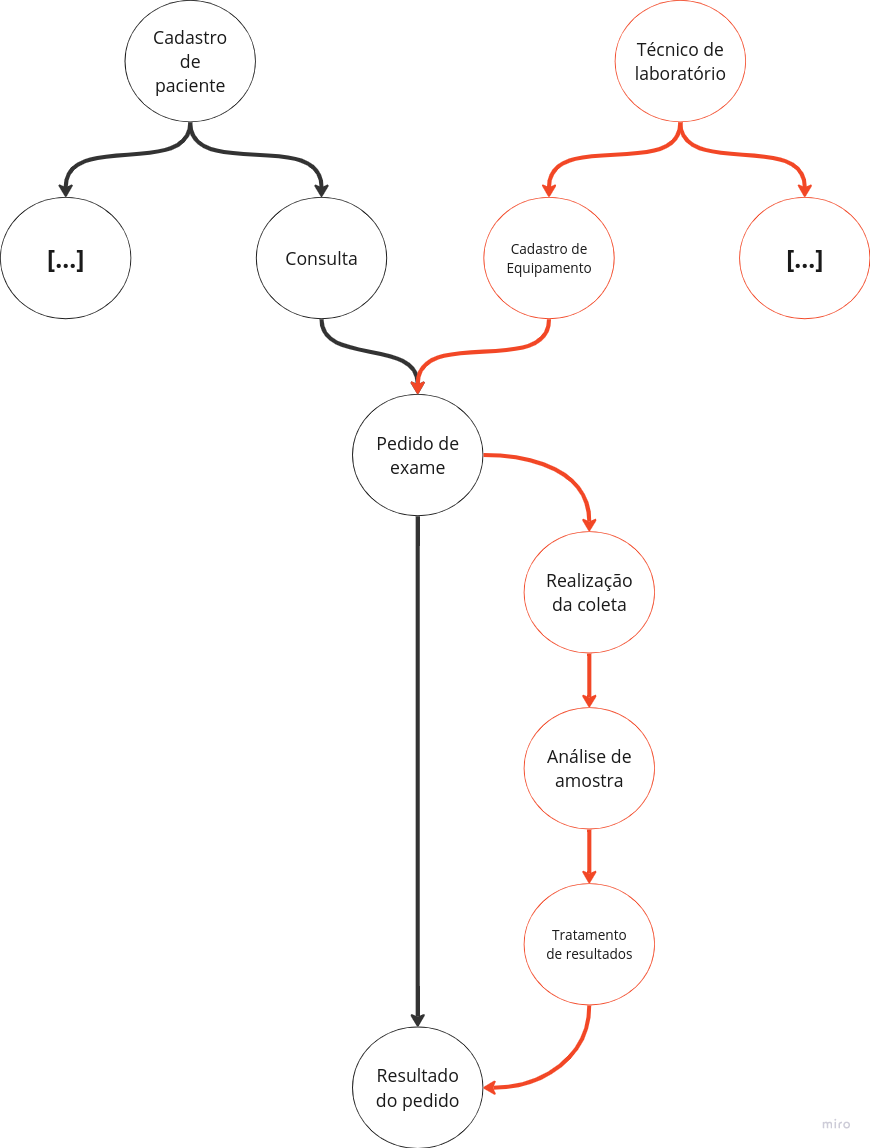
\includegraphics[width=0.65\textwidth]{imgs/Exemplo/exemplo_pedido_exame.png}
    \caption{Representação da implementação de múltiplas atividades iniciais. Neste exemplo, temos a instância de pacientes em preto e em vermelho temos o workflow do técnico de laboratório. Podemos ver que as atividades em preto e vermelho são compartilhadas, e apenas o técnico tem permissão de visualização das atividades entre o pedido de exame e o resultado do pedido.}
    \label{fig:segunda_implementacao}
\end{figure}

% Workflow grande feito no Flux

\subsection{CTTX e BPL Equipamentos} \label{sec:cttx_bpl}

Um outro exemplo utiliza os workflows CTTX (Citotoxicidade) e BPL (Boas Práticas de Laboratório) - Equipamentos. Estes dois workflows necessitam de troca de informações entre eles: BPL - Equipamentos precisa informar sobre a calibração de equipamentos para utilização no workflow CTTX.

Para isso, foi aplicado a implementação de compartilhamento de atividades entre a atividade de calibração do equipamento, disponibilizando a atividade ``Leitura de Absorbância: Perfil Inicial de Citotoxicidade (Range Finder)'' somente após uma atividade calibração do equipamento (Como podemos ver na figura~\ref{fig:cttx_eqp_structure}).

Utilizando o sistema de permissões do Flux, é possível limitar o acesso de cada tipo de usuário (cientista, técnico de laboratório, gerente de laboratório) para que o usuário tenha acesso apenas a informações relevantes ao seu trabalho. Um usuário responsável pela leitura de absorbância terá permissão para visualizar a calibração dos equipamentos utilizados, mas ele não pode realizar nenhuma calibração.

O técnico de laboratório não poderá executar nenhuma leitura de absorbância, e também não terá permissão para visualizar as atividades, enquanto que um gerente de laboratório pode visualizar todas as informações colocadas nos workflows, podendo alterar o tipo de visualização usando a implementação de workflows dinâmicos para obter informações mais rapidamente.

\begin{figure}
    \centering
    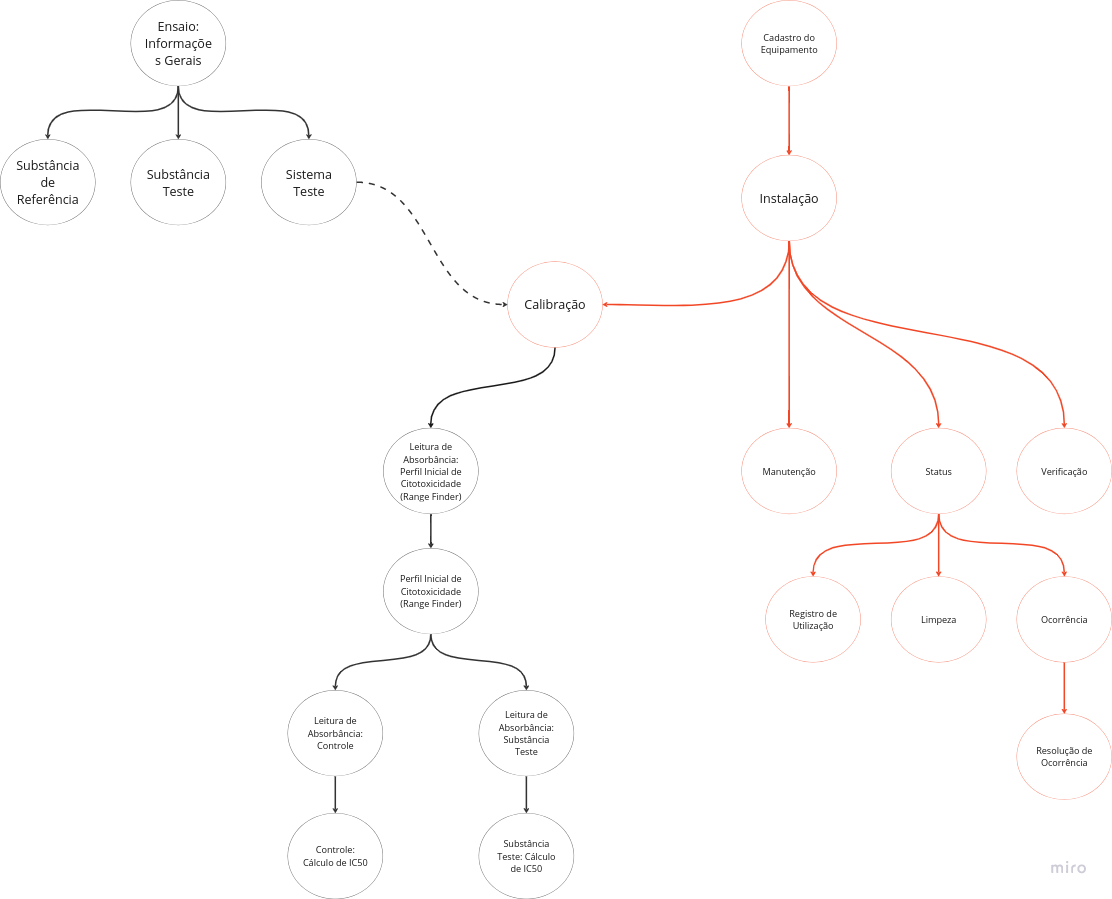
\includegraphics[width=1\textwidth]{imgs/CTTX-EQP/estrutura_cttx_eqp.png}
    \caption{Estrutura dos workflows CTTX e BPL-EQP. O workflow original do CTTX pode ser visto com as setas e círculos de cor preta. A seta pontilhada indica a transição antiga do workflow CTTX, sendo as novas transições entre ``Sistema Teste'' e ``Calibração'', e ``Calibração'' e ``Leitura de Absorbância: Perfil Inicial de Citotoxicidade (Range Finder)'' indicam as novas transições feitas para a comunicação da atividade ``Calibração'' do workflow BPL com o workflow CTTX. A atividade de Leitura de Absorbância só poderá ser realizada quando um equipamento for calibrado.}
    \label{fig:cttx_eqp_structure}
\end{figure}

O equipamento calibrado está identificado por um atributo dentro da atividade de calibração. Este atributo tem uma propriedade que faz o valor ser utilizado no nome da atividade. Caso o equipamento cadastrado tenha o nome de ``Balança Analítica'', a atividade de calibração terá o nome ``Calibração (Balança Analítica)'', com a data da calibração logo ao lado para maior facilidade de busca dos dados (como visto na imagem~\ref{fig:cttx_eqp_calibration}).

\begin{figure}
    \centering
    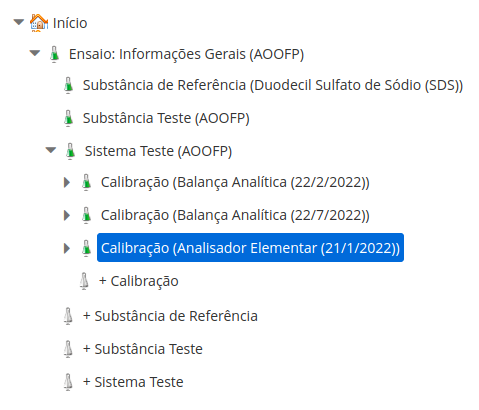
\includegraphics[width=.5\textwidth]{imgs/CTTX-EQP/calibration_tree.png}
    \caption{CTTX com as atividades de calibração de equipamento, identificadas pelo nome do equipamento e data de calibração.}
    \label{fig:cttx_eqp_calibration}
\end{figure}